\documentclass[12pt]{article}
\usepackage{ctex}
\usepackage{graphicx}
\usepackage{authblk}
\usepackage{subfigure}
\usepackage{caption}
\usepackage{amssymb}
\usepackage{graphicx, subfig}
\usepackage{float}
\usepackage{physics}
\usepackage{amsmath}
\usepackage{slashed}
\usepackage{geometry}
\captionsetup{font={small}}
\geometry{left=2.5cm,right=2.5cm,top=2.5cm,bottom=2.5cm}
\title{Deep-neural-network}
\date{}
\author[1]{Tingyu Zhang}
\affil[1]{Department of Physics, Graduate School of Science, The University of Tokyo, 
Tokyo 113-0033, Japan}
\graphicspath{{figures/}}

\begin{document}

\maketitle

\section{\large The Slater Jastrow Wave Function}

The Slater-Jastrow wave function can be written as
\begin{equation}\label{1}
    \Psi(\{\mathbf{r}_i\},\{\mathbf{R}_I\})=\exp\left[J(\{\mathbf{r}_i\},
    \{\mathbf{R}_I\})\right]D(\{\mathbf{r}_i\})
\end{equation}
where $\{\mathbf{r}_i\}$ and $\{\mathbf{R}_I\}$ denote the electron and nucleus 
coordinates, respectively. $\exp[J]$ is the Jastrow factor, and $D(\{\mathbf{r}_i\})$ 
denotes the Slater part, which only depends on the $\{\mathbf{r}_i\}$.

The Jastrow factor can be written as the sum of homogeneous, isotropic 
electron–electron terms $u$, isotropic electron–nucleus terms $\chi$ centered on the 
nuclei, isotropic electron–electron–nucleus terms $f$, also centered on the nuclei 
and, in periodic systems, plane-wave expansions of electron–electron separation 
and electron position, $p$ and $q$. The form is
\begin{equation}
    \begin{split}
        J\left(\left\{\mathbf{r}_{i}\right\},\left\{\mathbf{R}_{I}\right\}\right)
        =&\sum_{i=1}^{N-1} \sum_{j=i+1}^{N} u\left(r_{i j}\right)+\sum_{I=1}^M
        \sum_{i=1}^{N}\chi_{I}\left(r_{iI}\right)+\sum_{I=1}^M\sum_{i=1}^{N-1}
        \sum_{j=i+1}^{N}f_{I}\left(r_{iI},r_{jI},r_{ij}\right)\\
        &+\sum_{i=1}^{N-1}\sum_{j=i+1}^{N}p\left(\mathbf{r}_{ij}\right)
        +\sum_{i=1}^{N} q\left(\mathbf{r}_{i}\right)
    \end{split}
\end{equation}
where $N$ is the number of electrons and $M$ is the number of nuclei, 
$\mathbf{r}_{ij}=\mathbf{r}_i-\mathbf{r}_j$ and 
$\mathbf{r}_{iI}=\mathbf{r}_i-\mathbf{r}_I$.

\section{\large The Cusp Conditions}

When an electron approaches another electron or a nucleus of charge Z the potential 
energy contribution to the local energy $E_L$ diverges as $Z/r$, where r is the 
distance of two particles. The kinetic energy operator acting on the cusps
in the wave function must therefore supply an equal and opposite divergence in the 
local kinetic energy.
\subsection*{\normalsize The antiparallel-spin electron–electron cusp condition}

Consider the situation where two electrons of opposite spin, $i$ and $j$, approach 
one another and the wave functioncis non-zero at the two-particle coalescence point.
The cusp condition is
\begin{equation}\label{2}
    \left(\frac{\partial \hat{\Psi}}{\partial r_{i j}}\right)_{r_{i j}=0}=
    \frac{1}{2} \hat{\Psi}_{r_{i j}=0}
\end{equation} 
where we write the wave function in terms of center-of-mass and difference coordinates 
of electrons $i$ and $j$, $\bar{\mathbf{r}}_{ij}=(\mathbf{r}_i+\mathbf{r}_j)/2$ and 
$\mathbf{r}_{ij}=\mathbf{r}_i-\mathbf{r}_j$ and 
$\hat{\Psi}(\bar{\mathbf{r}}_{ij},r_{ij})$ is the spherical average of 
$\hat{\Psi}(\bar{\mathbf{r}}_{ij},\mathbf{r}_{ij})$ about the coalescence point. 
Neglecting the cuspless p and q terms, the Slater–Jastrow wave function may be 
written as
\begin{equation}
    \Psi\left(\overline{\mathbf{r}}_{ij},\mathbf{r}_{i j}\right)=\exp\left[J
    \left(r_{i},r_{j},r_{i j}\right)\right]D\left(\overline{\mathbf{r}}_{ij},
    \mathbf{r}_{i j}\right)
\end{equation}
to simplify, we assume there is only one nucleus located at the origin.
\begin{equation}
    \begin{split}
        \delta\Psi=&\Psi_{r_{ij}=0}\times\left(\left[\left(\frac{\partial J}{\partial
        r_i}\right)-\left(\frac{\partial J}{\partial r_j}\right)\right]_{r_{ij}=0}
        \delta r_i+\left(\frac{\partial J}{\partial r_{ij}}\right)_{r_{ij}=0}r_{ij}
        \right)\\
        &+\exp\left[J_{r_{ij}=0}\right]\left(\nabla_{ij} D\right)_{r_{ij}=0}
        \cdot\mathbf{r}_{ij}+\mathcal{O}\left(r_{ij}^{2}\right)
    \end{split}
\end{equation}
where $\delta\mathbf{r}_i$ and $\delta\mathbf{r}_j$ are the changes in $\mathbf{r}_i$ 
and $\mathbf{r}_j$ and $\delta\mathbf{r}_i=-\delta\mathbf{r}_j$.  If the spherical 
average about the coalescence point is taken then the terms involving $\delta r_i$ 
and $\mathbf{r}_{ij}$ vanish to $\mathcal{O}(r_{ij})$, so that
\begin{equation}
    \delta \hat{\Psi}=\hat{\Psi}_{r_{i j}=0}\left(\frac{\partial J}{\partial r_{i j}}
    \right)_{r_{i j}=0}r_{i j}+\mathcal{O}\left(r_{i j}^{2}\right)
\end{equation} 
Also notice that 
\begin{equation}
    \begin{split}
        \delta\hat{\Psi}&=\left(\frac{\partial \hat{\Psi}}{\partial r_{i j}}
        \right)_{r_{i j}=0}r_{ij}=\frac{1}{2} \hat{\Psi}_{r_{i j}=0}r_{ij}\\
        &=\hat{\Psi}_{r_{i j}=0}\left(\frac{\partial J}{\partial r_{i j}}
        \right)_{r_{i j}=0}r_{i j}+\mathcal{O}\left(r_{i j}^{2}\right)
    \end{split}
\end{equation}
Therefore the antiparallel cusp condition is equivalent to
\begin{equation}
    \left(\frac{\partial J}{\partial r_{i j}}\right)_{r_{i j}=0 \atop r_{i}=r_{j}}
    =\frac{1}{2}
\end{equation}
\subsection*{\normalsize The parallel-spin electron–electron cusp condition}
The cusp condition for electrons $i$ and $j$ with parallel spins is 
\begin{equation}\label{3}
    \left(\frac{\partial \Psi_{1 m}}{\partial r_{i j}}\right)_{r_{i j}=0}=
    \frac{1}{4}\left(\Psi_{1 m}\right)_{r_{i j}=0}.
\end{equation}
where $\Psi_{1m}$ is the $r_{ij}Y_{1m}$ component of $\Psi$, and $Y_{1m}$ is the 
$(1,m)$th spherical harmonic.
This cusp condition is equivalent to the requirement that
\begin{equation}
    \left(\frac{\partial J}{\partial r_{i j}}\right)_{r_{i j}=0 
    \atop r_{i}=r_{j}}=\frac{1}{4}
\end{equation}
\subsection*{\normalsize The electron–nucleus cusp condition}

The cusp condition for a electron $i$ approaching a nucleus of atomic number Z is
\begin{equation}
    \left(\frac{\partial\bar{\Psi}}{\partial r_i}\right)_{r_i=0}=-Z\bar{\Psi}_{r_i=0}
\end{equation}
where $\bar{\Psi}(r_i)$ is The spherical average of $\Psi(r_i)$ about the nucleus.
if the Slater determinant is continuously differentiable at the nucleus then the 
Jastrow factor must satisfy
\begin{equation}
    \left(\frac{\partial J}{\partial r_{i j}}\right)_{r_i=0 
    \atop r_{ij}=r_{j}}=-Z.
\end{equation}
If the Slater part of the wave function satisfies the electron–nucleus cusp condition, 
or if a non-divergent pseudopotential is used, then the Jastrow factor is required 
to be cuspless at the nuclei. 

\section{\large Backflow Transformation}

The Slater-Jastrow wave function is written as Eq.(\ref{1}). After backflow 
transformation, the wave function becomes
\begin{equation}
    \Psi^{\rm BF}(\{\mathbf{r}_i\},\{\mathbf{R}_I\})=\exp\left[J(\{\mathbf{r}_i\},
    \{\mathbf{R}_I\})\right]D(\{\mathbf{X}\})
\end{equation}
where $\mathbf{X}=\{\mathbf{x}_{i}\}$ is a set of \emph{collective coordinates},
\begin{equation}
    \mathbf{x}_{i}=\mathbf{r}_i+\boldsymbol{\xi}_{i}(\mathbf{r},\mathbf{R}),
\end{equation}
where $\boldsymbol{\xi}_{i}$ is the backflow displacement of electron $i$, which depends on 
the configuration of the whole system. The electron–electron contribution to the 
backflow displacement $\boldsymbol{\xi}_{i}$ is 
\begin{equation}
    \boldsymbol{\xi}_{i}^{\mathrm{ee}}=\sum_{j\neq i}^N\eta_{ij}\mathbf{r}_{ij}
\end{equation}
where $N$ is the number of electrons and $\eta_{ij}= \eta(r_{ij})$ is a function of the 
interparticle distance $r_{ij}$. The electron–nucleus contribution to the 
backflow displacement $\boldsymbol{\xi}_{i}$ is
\begin{equation}
    \boldsymbol{\xi}_{i}^{\mathrm{en}}=\sum_{I}^M\mu_{iI}\mathbf{r}_{iI}
\end{equation}
where $\mu_{iI}=\mu(r_{iI})$ and $M$ is the number of nuclei. 

Also, there is an electron-electron-nucleus term to describe two-electron backflow 
displacements in the presence of a nearby nucleus,
\begin{equation}
    \boldsymbol{\xi}_{i}^{\rm een}=\sum_{j\neq i}^N\sum_{I}^M\left(\Phi_i^{jI}
    \mathbf{r}_{ij}+\Theta_i^{jI}\mathbf{r}_{iI}\right)
\end{equation}
where $\Phi^{jI}_i=\Phi^I(r_{iI},r_{jI},r_{ij})$ and $\Theta^{jI}_i=\Theta^I(r_{iI},r_{jI},r_{ij})$. 
Since the vector $\Phi_i^{jI}\mathbf{r}_{ij}+\Theta_i^{jI}\mathbf{r}_{iI}$ is 
able to span the plane defined by $\mathbf{r}_i$, $\mathbf{r}_j$ and $\mathbf{r}_I$, 
there is no need to introduce a component along the direction of $\mathbf{r}_{jI}$. 
The total backflow displacement is the sum of these three components,
\begin{equation}
    \boldsymbol{\xi}_{i}=\boldsymbol{\xi}_{i}^{\rm ee}+\boldsymbol{\xi}_{i}^{\rm en}
    +\boldsymbol{\xi}_{i}^{\rm een}
\end{equation}

\section{\large DNN electronic wavefunction ansatz}

In this work, the PauliNet, a deep learning QMC approach is developed by replacing 
existing ad hoc functional forms used in the standard Jastrow factor and backflow 
transformation with more powerful deep neural network (DNN) representations. Using 
this approach, for systems with a few tens of electrons, we can obtain high accuracy 
with orders of magnitude fewer determinants compared to traditional QMC methods.
(Fig.\ref{img1})
\begin{figure}[H]
    \centering
    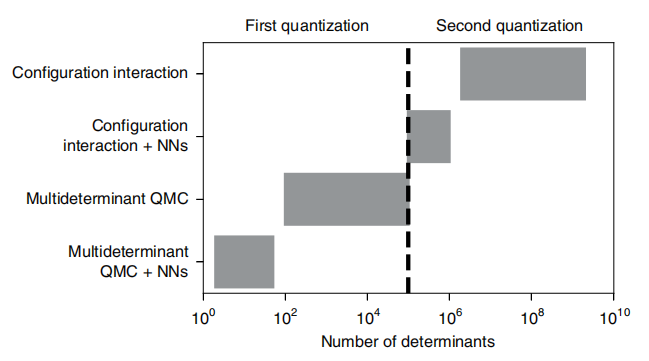
\includegraphics[width=13cm]{p1.png}
    \renewcommand{\figurename}{Fig.}
    \caption{Combinatorial explosion of the number of Slater determinants in 
    quantum chemistry.This figure shows typical numbers of Slater determinants 
    used by high-accuracy quantum chemistry methods in state-of-the-art 
    calculations on atomic systems with at most a few tens of electrons.}
    \label{img1}
\end{figure}

At the core of the deep-learning approach to the electronic Schrödinger equation is 
a wavefunction ansatz, named PauliNet, which incorporates both the well-established 
essential physics of electronic wavefunctions, which contains Slater determinants, 
multideterminant expansion, Jastrow factor, backflow transformation and cusp 
conditions, as well as DNNs capable of encoding the complex features of the 
electronic motion. Our proposed trial wavefunction is of the multideterminant 
Slater–Jastrow–backflow type: 
\begin{equation}
    \begin{split}
        &\psi_{\boldsymbol{\theta}}(\mathbf{r})=\mathrm{e}^{\gamma(\mathbf{r})+
        J_{\boldsymbol{\theta}}(\mathbf{r})}\sum_{p} c_{p} \operatorname{det}
        \left[\tilde{\varphi}_{\boldsymbol{\theta}, \mu_{p} i}^{\uparrow}(\mathbf{r})
        \right] \operatorname{det}\left[\tilde{\varphi}_{\boldsymbol{\theta},\mu_{p}i}
        ^{\downarrow}(\mathbf{r})\right]\\
        &\tilde{\varphi}_{\mu i}(\mathbf{r})=\varphi_{\mu}(\mathbf{r}_{i})
        f_{\boldsymbol{\theta},\mu i}(\mathbf{r})
    \end{split}
\end{equation}
where $\textbf{r}=(\textbf{r}_1\cdots\textbf{r}_N)$ and both the Jastrow factor J 
and backflow function $\textbf{f}$ are represented by DNNs with trainable parameters 
$\boldsymbol{\theta}$.(Fig.\ref{img2})

The electronic cusp conditions are enforced by $\gamma(\mathbf{r})$ to satisfy the 
cusp condition (Eq.\ref{2} and Eq.\ref{3}),
\begin{equation}
    \gamma(\mathbf{r}):=\sum_{i<j}-\frac{c_{i j}}{1+\left|\mathbf{r}_{i}-
    \mathbf{r}_{j}\right|}
\end{equation}
where $c_{ij}$ is $\frac{1}{2}$ for electrons with opposite spins and $\frac{1}{4}$ 
for electrons with the same spin. Besides, the nuclear cusp conditions are built in 
$\varphi_{\mu}(\mathbf{r}_i)$. To preserve the cusp conditions built into 
$\varphi_\mu$ and $\gamma$, the Jastrow factor and backflow DNNs must be cuspless,
\begin{equation}
    \left.\nabla_{\mathbf{r}_{i}} J(\mathbf{r})\right|_{\mathbf{r}_{i}=
    \left\{\mathbf{r}_{k}, \mathbf{R}_{I}\right\}}=0,\left.\quad 
    \nabla_{\mathbf{r}_{i}} f_{\mu i}(\mathbf{r})\right|_{\mathbf{r}_{i}=
    \left\{\mathbf{r}_{k}, \mathbf{R}_{t}\right\}}=0
\end{equation}

PauliNet uses an adapted form of one such DNN architecture, called SchNet, which  
represents each particle with a vector in a high-dimensional abstract 
feature space, $\mathbf{x}_i$, which is iteratively refined by interactions with 
other particles through real-space trainable convolutions, $\chi_{\boldsymbol{\theta}}$.
\begin{equation}
    \mathbf{x}_{i}^{(n+1)}:=\mathbf{x}_{i}^{(n)}+\chi_{\boldsymbol{\theta}}^{(n)}\left(\left
    \{\mathbf{x}_{j}^{(n)},\left\{\left|\mathbf{r}_j-\mathbf{r}_{k}\right|\right\}
    \right\}\right).
\end{equation}
In PauliNet we implement the following interation rule
\begin{equation}
    \begin{array}{l}
        \mathbf{z}_i^{(n,\pm)}:=\sum_{j\neq i}^\pm\mathbf{w}_{\boldsymbol{\theta}}^{(n,\pm)}
        \left(\mathbf{e}\left(\left|\mathbf{r}_i-\mathbf{r}_j\right|\right)\right)
        \odot \mathbf{h}_{\boldsymbol{\theta}}^{(n)}\left(\mathbf{x}_{j}^{(n)}\right)\\
        \mathbf{z}_i^{(n,\mathrm{n})}:=\sum_I\mathbf{w}_{\boldsymbol{\theta}}^{(n,\mathrm{n})}
        \left(\mathbf{e}\left(\left|\mathbf{r}_i-\mathbf{R}_I\right|\right)\right)
        \odot \mathbf{Y}_{\boldsymbol{\theta}, I}\\
        \mathbf{x}_i^{(n+1)}:=\mathbf{x}_i^{(n)}+\sum_\pm\mathbf{g}_{\boldsymbol{\theta}}^{(n,\pm)}
        \left(\mathbf{z}_i^{(n,\pm)}\right)+\mathbf{g}_{\boldsymbol{\theta}}^{(n,n)}
        \left(\mathbf{z}_{i}^{(n,\mathrm{n})}\right)
        \end{array}
\end{equation}
where `$\odot$' denotes element-wise multiplication and $\mathbf{w}_{\boldsymbol{\theta}}$, 
$\mathbf{h}_{\boldsymbol{\theta}}$, $\mathbf{g}_{\boldsymbol{\theta}}$ are trainable functions represented by 
ordinary fully connected DNNs; and $\mathbf{e}$ is a radial basis function that 
featurizes the interatomic distances. The messages $z_i^{(n)}$ received by the 
electron feature vectors at each iteration are split into three channels, 
corresponding to same-spin electrons $(+)$, opposite-spin electrons $(−)$ and 
the nuclei $(n)$. Besides, each channel has a separate receiving function gθ, 
again increasing fexibility without substantially increasing the number of 
parameters.
\begin{figure}[H]
    \centering
    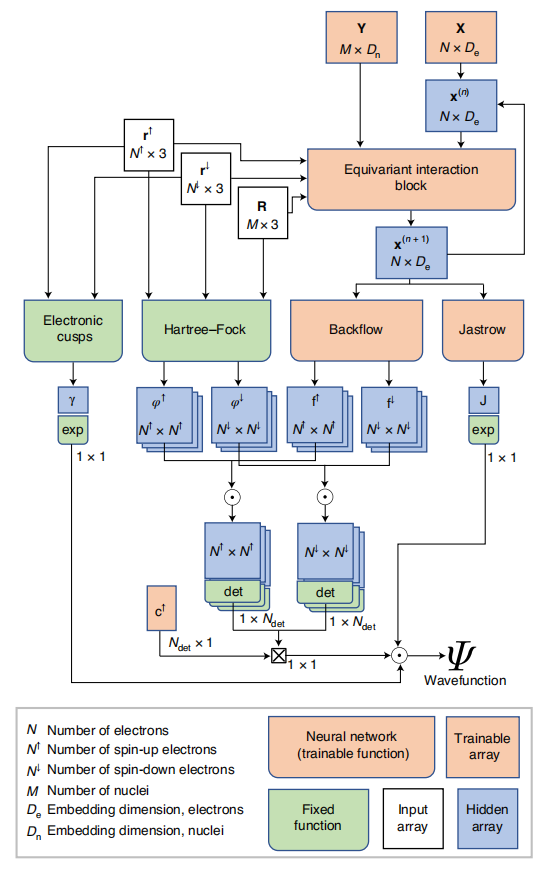
\includegraphics[width=11cm]{p2.png}
    \renewcommand{\figurename}{Fig.}
    \caption{Architecture of the newly developed PauliNet wavefunction ansatz. 
    The information flows from the input electron and nuclear coordinates, 
    $\mathbf{r}$ and $\mathbf{R}$, to the output wavefunction value, $\Psi$.}
    \label{img2}
\end{figure}

We expand the distances in a basis of Gaussians, which are modified to forces all 
the features and their derivatives to zero at zero distance,
\begin{equation}
    \begin{array}{l}
        e_{k}(r):=r^{2} \mathrm{e}^{-r-\left(r-\mu_{k}\right)^{2}/\sigma_{k}^{2}}\\
        \mu_{k}:=r_{\mathrm{c}} q_{k}^{2},\quad\sigma_{k}:=\frac{1}{7}
        \left(1+r_{\mathrm{c}} q_{k}\right)
        \end{array}
\end{equation}
where $q_k$ equidistantly spans the interval $(0, 1)$ and $r_c$ is the cutoff 
distance.

After a fixed number of iterations, the final electron representations, $x_i^{(L)}$, 
which now encode complex many-body electron correlations, are used as an input to 
two trainable functions, $\eta_\theta$ and $\kappa_\theta$, which return the 
Jastrow factor and backflow, respectively:
\begin{equation}
    J:=\eta_{\theta}\left(\sum_{i} \mathbf{x}_{i}^{(L)}\right), \quad 
    \mathbf{f}_{i}:=\boldsymbol{\kappa}_{\theta}\left(\mathbf{x}_{i}^{(L)}\right)
\end{equation}
Since the feature vectors $\mathbf{x}_i^{(n)}$ are equivariant with respect to electron 
exchange at each iteration, we can easily prove that the Jastrow factor $J$ is 
invariant while the backflow vectors $\mathbf{f}_i$ are equivariant with respect 
to exchanges of electrons.
\begin{equation}
    J\left(\mathcal{P}_{ij}\mathbf{r}\right)=J(\mathbf{r}),\quad\mathcal{P}_{ij}
    f_{\mu i}(\mathbf{r})=f_{\mu j}\left(\mathcal{P}_{ij}\mathbf{r}\right),
\end{equation}
where $\mathcal{P}_{ij}$ is the exchange of same-spin electrons $i$ and $j$. 
Therefore the PauliNet wave function is constructed to be antisymmetric,
\begin{equation}
    \psi_\theta\left(\ldots, \mathbf{r}_{i}, \ldots, \mathbf{r}_{j}, \ldots\right)=
    -\psi_\theta\left(\ldots, \mathbf{r}_{j}, \ldots, \mathbf{r}_{i}, \ldots\right).
\end{equation}
\section{\large Approaching exact solutions with few determinants}
We train PauliNet via the variational principle, minimizing the total electronic 
energy (variational QMC).
\begin{equation}
    E_{0}=\min _{\psi} E[\psi] \leq \min _{\theta} E\left[\psi_{\theta}\right],
\end{equation}
where 
\begin{equation}
    E[\psi]=\int \mathrm{d} \mathbf{r} \psi^{\dagger}(\mathbf{r}) \hat{H} \psi(\mathbf{r})
\end{equation}
Following the standard QMC technique, the energy integral is evaluated as an 
expected value of the local energy 
$E_{\rm loc}[\psi](\mathbf{r})=\{\hat{H}\psi(\mathbf{r})\}/\psi(\mathbf{r})$, over the 
probability distribution $|\psi(\mathbf{r})|^2$,
\begin{equation}
    E[\psi]=\mathbb{E}_{\mathbf{r}\sim|\psi|^2}[E_{\rm loc}[\psi](\mathbf{r})]
\end{equation}
To optimize the parameters $\boldsymbol{\theta}$ in the Jastrow and backflow neural networks, we 
use the weighted Adam algorithm:

\hrulefill
\begin{center}
    \begin{tabular}{l}
        \textbf{Require:} $\alpha$: Stepsize\\
        \textbf{Require:} $\beta_1,\beta_2\in [0,1)$: Exponential decay rates for 
        the moment estimates\\
        \textbf{Require:} $f(\theta)$:  Stochastic objective function with 
        parameters $\theta$\\
        \textbf{Require:} $\theta_0$: Initial parameter vector\\
        \ \ $m_0\leftarrow0$ \ (Initialize $\rm 1^{st}$ moment vector)\\
        \ \ $v_0\leftarrow0$  \ (Initialize $\rm 2^{nd}$ moment vector)\\
        \ \ $t\leftarrow0$  (Initialize timestep)\\
        \ \ \textbf{while} $\theta_t$ not converged \textbf{do}\\
        \ \ \ \ $t\leftarrow t+1$\\
        \ \ \ \ $g_t\leftarrow\nabla_\theta f_t(\theta_{t-1})$ \ (Get gradients 
        w.r.t. stochastic objective at timestep)\\
        \ \ \ \ $m_t\leftarrow\beta_1\cdot m_{t-1}+(1-\beta_1)\cdot g_1$ \ (Update biased 
        first moment estimate)\\
        \ \ \ \ $v_t\leftarrow\beta_2\cdot v_{t-1}+(1-\beta_2)\cdot g_1^2$ \ (Update 
        biased second raw moment estimate)\\
        \ \ \ \ $\hat{m}_t\leftarrow m_t/(1-\beta_1^t)$ \ (Compute bias-corrected first 
        moment estimat)\\
        \ \ \ \ $\hat{v}_t\leftarrow v_t/(1-\beta_2^t)$ \ (Compute bias-corrected second 
        raw moment estimate)\\
        \ \ \ \ $\theta_t\leftarrow \theta_{t-1}-\alpha\cdot\hat{m}_t/(\sqrt
        {\hat{v}_t}+\varepsilon)$ \ (Update parameters)\\
        \ \ \textbf{end while}\\
        \ \ \textbf{return} $\theta_t$ \ (Resulting parameters)
    \end{tabular}
\end{center}

\hrulefill

In the algorithm above, $g^2_t$ indicates the elementwise square $g_t\odot g_t$, 
and $\beta_1^t$ and $\beta_2^t$ denote $\beta_1$ and $\beta_2$ to the power of $t$. 
Besides, we use the total energy directly as the loss function,
\begin{equation}
    \mathcal{L}(\boldsymbol{\theta})=\mathbb{E}_{\mathbf{r}\sim\left|\psi_\theta
    \right|^2}\left[E_{\operatorname{loc}}\left[\psi_{\theta}\right](\mathbf{r})\right].
\end{equation}
To calculate the 
stochastic gradient of the loss function over a batch of samples, we use a gradient 
formula that takes advantage of the fact that the Hamiltonian operator is Hermitian.
Since 
\begin{equation}
    \begin{split}
        \frac{\partial}{\partial\theta}\mathbb{E}_{\mathbf{r}\sim p(\mathbf{r};\theta)}
        [f(\mathbf{r};\theta)]&=\frac{\partial}{\partial\theta}\int d^3rp(\mathbf{r};\theta)
        f(\mathbf{r};\theta)\\
        &=\int d^3r\left[\frac{\partial p(\mathbf{r};\theta)}{\partial\theta}
        f(\mathbf{r};\theta)+p(\mathbf{r};\theta)\frac{\partial f(\mathbf{r};\theta)}
        {\partial\theta}\right]\\
        &=\int d^3r\left[p(\mathbf{r};\theta)\frac{\partial \ln p(\mathbf{r};\theta)}
        {\partial\theta}f(\mathbf{r};\theta)+p(\mathbf{r};\theta)\frac{\partial 
        f(\mathbf{r};\theta)}{\partial\theta}\right]\\
        &=\mathbb{E}_{\mathbf{r}\sim p(\mathbf{r};\theta)}\left[\left(\frac{\partial}
        {\partial\theta}\ln p(\mathbf{r};\theta)\right)f(\mathbf{r};\theta)+
        \frac{\partial}{\partial \theta}f(\mathbf{r};\theta)\right],
    \end{split}
\end{equation}
Therefore we can write the gradient of the loss function w.r.t. $\mathbf{\theta}$:
\begin{equation}
    \nabla_{\theta}\mathcal{L}(\boldsymbol{\theta})=2\mathbb{E}_{\mathbf{r}
    \sim\left|\psi_\theta\right|^2}[E_{\operatorname{loc}}[\psi_{\theta}]
    (\mathbf{r})\nabla_{\boldsymbol{\theta}}\ln|\psi_{\theta}|]-2\mathcal{L}
    (\boldsymbol{\theta})\mathbb{E}_{\mathbf{r}\sim\left|\psi_\theta\right|^2}
    [\ln|\psi_{\theta}|].
\end{equation}
This expression for the gradient requires calculating only second derivatives 
of the wavefunction (for the Laplace operator), whereas direct differentiation 
would require third derivatives (derivative of the Laplace operator).
\section{\large Performance of PauliNet on some small moleculars}
They first investigate the hydrogen molecule ($\rm H_2$), lithium hydride (LiH), 
beryllium (Be), boron (B) and the linear hydrogen chain $\rm H_{10}$. For the 
mono- and diatomic systems, PauliNet reaches the correlation energy between 
$97\%$ and $99.9\%$ with one to two orders of magnitude less determinants than 
standard variational ansatzes (Fig.\ref{img3}).
\begin{figure}[H]
    \centering
    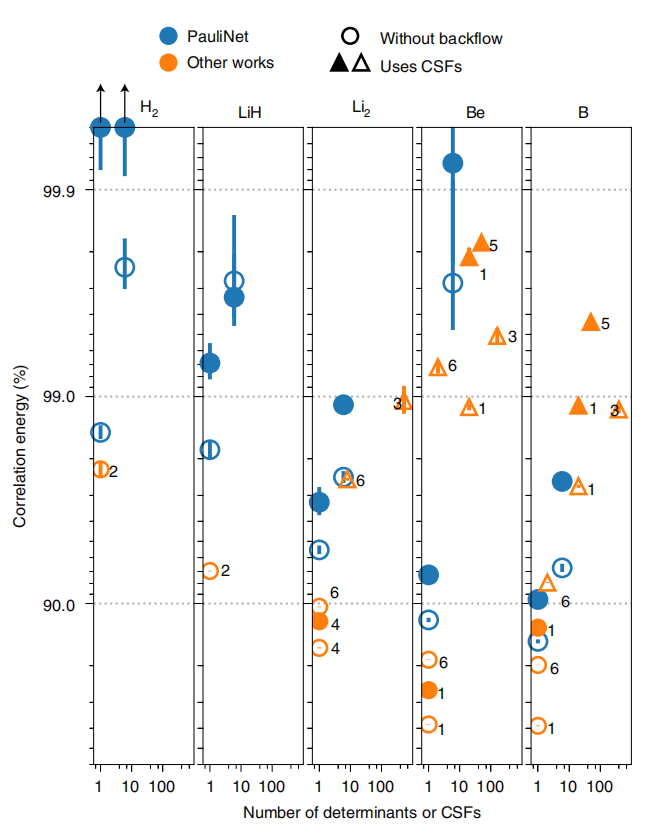
\includegraphics[width=10cm]{p3.png}
    \renewcommand{\figurename}{Fig.}
    \caption{Performance of PauliNet with one and six determinants on atoms and 
    diatomic molecules. Four variants of PauliNet are shown, single and 
    multideterminant as well as with and without backflow. The reference 
    results are taken from (1) Brown et al., (2) Casalegno et al., (3) Morales 
    et al., (4) Lopez Ríos et al., (5) Seth et al. and (6) Toulouse and Umrigar.}
    \label{img3}
\end{figure}

Four variants with a single or multiple Slater determinant(s) (SD or MD), 
with or without backflow (BF) are shown in Fig.\ref{img4}, which shows that both 
the backflow and the use of a few determinants is crucial for reaching high accuracy.
\begin{figure}[H]
    \centering
    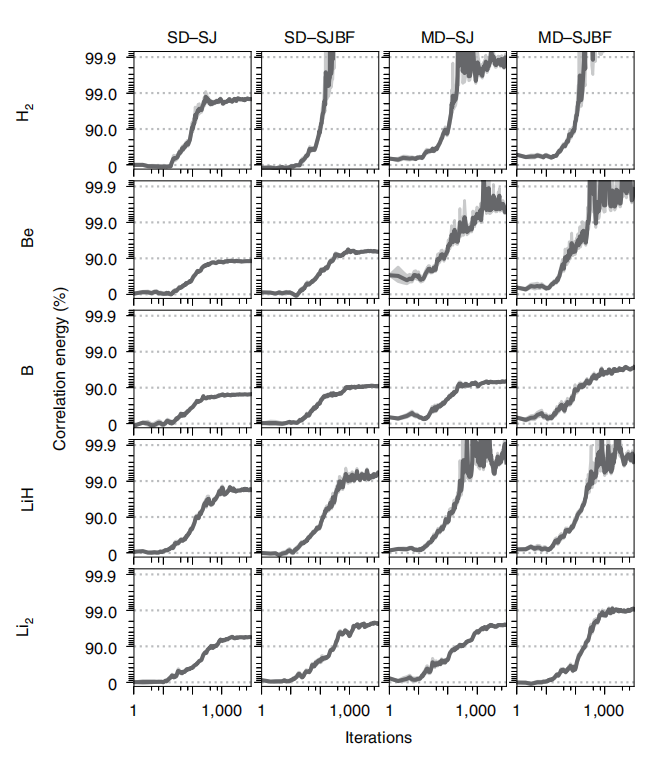
\includegraphics[width=13cm]{p4.png}
    \renewcommand{\figurename}{Fig.}
    \caption{Roles of backflow and multiple determinants in training of PauliNet 
    ansatz.}
    \label{img4}
\end{figure}

For linear hydrogen chain $\rm H_{10}$ which exhibits strong correlation, they recover 
$98.41(8)\%$ and $98.4(3)\%$ of the correlation energy in the equilibrium and 
stretched geometries, respectively, using 16 determinants (Fig.\ref{img5}). The 
results are only slightly worse using a single determinant (98.10(9)\% and 97.5(4)\%), 
but substantially worse when the trainable backflow is also switched off (93.7(2)\% 
and 82(2)\%), which indicates that the backflow plays a much larger role than 
multiple determinants in this strong correlation system,  highlighting the central 
role of the trainable backflow in PauliNet. 
\begin{figure}[H]
    \centering
    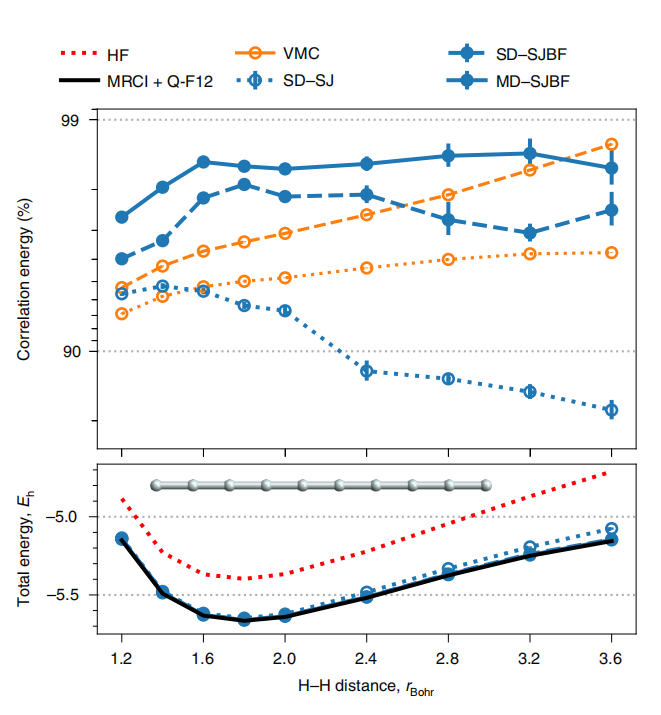
\includegraphics[width=13cm]{p5.png}
    \renewcommand{\figurename}{Fig.}
    \caption{The correlation energy recoverd in linear hydrogen chain $\rm H_{10}$. 
    PauliNet results (blue) with single determinant or 16 determinants (MD) and 
    with or without backflow are shown. The correlation energy is calculated with 
    respect to multireference configuration-interaction (MRCI) results. $E_h$, 
    Hartree energy; $r_{Bohr}$, Bohr radius.}
    \label{img5}
\end{figure}
\section{\large Straightforward generalization to larger molecules}
The automerization of cyclobutadiene (环丁二烯) (Fig.\ref{img6}a, 28 electrons) is a chemical 
process that has received considerable attention from both experiment and theory.
The experimental estimates of the energy barrier range between 1.6 and 10 
kcal$\cdot\rm mol^{-1}$. However, the standard coupled-cluster method with up to 
perturbative triple excitations (CCSD(T)) predicts 18 $\rm kcal\cdot mol^{-1}$, a twofold 
overestimation.The best computational estimates are available from various flavours 
of the multireference coupled-cluster (MR-CC) theory and fall between 7 and 
11 $\rm kcal\cdot mol^{-1}$, without a decisive answer as to which of the variants is 
closer to the ground truth.
\begin{figure}[H]
    \centering
    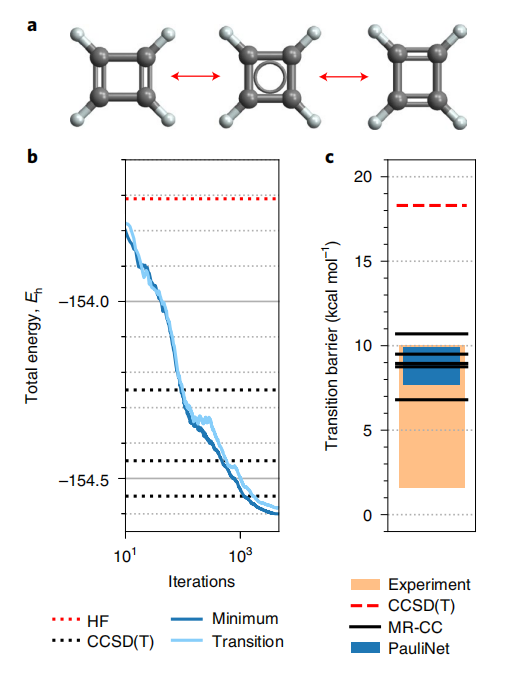
\includegraphics[width=11cm]{p6.png}
    \renewcommand{\figurename}{Fig.}
    \caption{Calculation of the transition barrier of cyclobutadiene automerization. 
    \textbf{a}, Cyclobutadiene automerization. The transition state has a highly 
    multireferential character. \textbf{b}, Convergence of the total energy of the 
    energy minimum and transition state with training. \textbf{c}, Energy barrier 
    obtained by sampling the trained PauliNet wavefunctions, compared with results 
    obtained by other approaches.}
    \label{img6}
\end{figure}

The PauliNet ansatz with ten determinants and the same hyperparameters as used 
for the much smaller systems is able to give all-electron variational energies for the 
energy minimum and transition states of cyclobutadiene, and thus for the energy 
barrier (Fig.\ref{img6}b).

\end{document}